\documentclass{beamer}
\usepackage{booktabs}
\usepackage{pdfpages}
\usepackage{mathtools}
\usepackage{enumerate}
\usepackage{multirow,tabularx}
\usepackage{booktabs}
\usepackage{pdfpages}
\usepackage{proof}
\usepackage{cancel}
\usepackage{chronology}
\usepackage{graphicx}
\usepackage{ulem}
\usepackage{amsmath}
\usepackage{amssymb}
\usepackage{color}
\usepackage{animate}
\usepackage{xr}

\PassOptionsToPackage{usenames,dvipsnames,svgnames}{xcolor}  
\usepackage{tikz}
\usepackage{tkz-graph}


\usepackage{wasysym}
\usepackage{proof}
\usepackage{cancel}
\usepackage{chronology}
\usepackage{graphicx}
\usepackage{ulem}
\usepackage{amsmath}
\usepackage{amssymb}
\usepackage{color}
\usepackage{xcolor}
\usepackage{soul}
%\usepackage{pstricks}
\setbeamertemplate{navigation symbols}{}

\newcommand{\norm}[1]{\left\lVert#1\right\rVert}
\newcommand{\el}{$\mathcal{EL}^{++}$}
\renewcommand{\Re}{\mathbb{R}}
\newcommand{\BigO}[1]{\ensuremath{\operatorname{O}\bigl(#1\bigr)}}
\newcommand{\myul}[2][blue]{\sethlcolor{#1}\hl{#2}\setulcolor{black}}

\newcommand<>{\cunderline}[3]{\only<#1>{#3}\only<#2>{\underline{#3}}}
\newcommand<>{\cem}[3]{\only<#1>{#3}\only<#2>{\ul{#3}}}
\newcommand<>{\cgray}[3]{\only<#1>{#3}\only<#2>{\textcolor{gray}{#3}}}
\newcommand<>{\colorize}[4]{\only<#1>{#4}\only<#2>{\textcolor{#3}{#4}}}

\setbeamertemplate{navigation symbols}{\insertslidenavigationsymbol}
%\setbeamertemplate{navigation symbols}{}
% \addtobeamertemplate{navigation symbols}{}{%
%     \usebeamerfont{footline}%
%     \usebeamercolor[fg]{footline}%
%     \hspace{1em}%
%     \insertframenumber/\inserttotalframenumber
% }

\mode<presentation>
{
\usecolortheme{crane}
%\useoutertheme{split}

\expandafter\def\expandafter\insertshorttitle\expandafter{%
  \insertshorttitle\hfill%
  \insertframenumber\,/\,\inserttotalframenumber}

\usefonttheme[onlysmall]{structurebold}
}
\renewcommand{\em}{\itshape}
\usepackage{pifont}
\definecolor{purple}{rgb}{1,0,1}
\definecolor{dred}{rgb}{0.7,0,0}
\definecolor{myred}{rgb}{1,0,0}
\definecolor{dblue}{rgb}{0,0,0.7}
\definecolor{dgreen}{rgb}{0,0.5,0}
\definecolor{myyellow}{rgb}{1,1,0}
\newcommand{\parents}[1]{parents(#1)}
\setbeamertemplate{itemize item}[ball]


% \mode<presentation>
% {
% \useinnertheme[shadow=true]{rounded}
% \useoutertheme{infolines}
% \usecolortheme{dove}
% \setbeamerfont{block title}{size={}}
% }

\title[Bio-Ontologies]{Embeddings for Description Logic}

\author{Robert Hoehndorf}


\date{}

\begin{document}

\begin{frame}
  \titlepage
\end{frame}

\begin{frame}
  \frametitle{Description Logics: overview}
  \begin{itemize}
  \item TBox: axioms pertaining to the terminology of the domain (classes)
  \item ABox: axioms stating facts (assertions) about the world
  \item RBox: axioms holding for relations
  \item Reasoning: derive implicitly represented knowledge (e.g.,
    subsumption)
  \item NB: a ``knowledge graph'' is an ABox + RBox
  \end{itemize}
\end{frame}

\begin{frame}
  \frametitle{Manchester OWL Syntax}
  \begin{table}[ht]
    \centering
    \begin{tabular}{|l|l|l|}
      DL Syntax & Manchester Syntax & Example \\
      \hline
      $C \sqcap D$ & C and D & Human and Male \\
      $C \sqcup D$ & C or D & Male or Female \\
      $\neg C$ & not C & not Male \\
      $\exists R.C$ & R some C & hasChild some Human \\
      $\forall R.C$ & R only C & hasChild only Human \\
      $(\geq n R.C)$ & R min n C & hasChild min 1 Human \\
      $(\leq n R.C)$ & R max n C & hasChild max 1 Human \\
      $(= n R.C)$ & R exactly n C & hasChild exactly 1 Human \\
      $\{a\} \sqcup \{b\} \sqcup ...$ & \{a b ...\} & \{John Robert
                                                      Mary\} \\
      \hline
    \end{tabular}
  \end{table}
\end{frame}

\begin{frame}
  \frametitle{Ontology embeddings}
  \begin{itemize}
  \item embedding methods for ontologies can be graph-based,
    language-based, or model-based 
    \begin{enumerate}
    \item graph-based: ontology as a graph
    \item text-based: extract (or obtain) text for classes/relations
    \item model-based: define embedding directly on
      $\Sigma$-structures
    \end{enumerate}
  \item for (1) we need to generate graphs from ontologies
    \begin{itemize}
    \item {\em is-a} relations are easy (this is just {\tt
        owl:subClassOf}) 
    \item how about {\em part-of}, {\em regulates}, {\em precedes},
      etc.?
    \item disjointness, universal vs. existential quantification,
      cardinality restrictions, intersection, union, negation?
    \end{itemize}
  \item relational patterns are implicit in OWL axioms
    \begin{itemize}
    \item design patterns as ``relations'' between classes
    \end{itemize}
  \end{itemize}
\end{frame}

\begin{frame}
  \frametitle{Relations as patterns}
  \begin{itemize}
  \item {\tt X SubClassOf: Y}: $X \xrightarrow{\text{is-a}} Y$
  \item {\tt X SubClassOf: part-of some Y}: $X \xrightarrow{\text{part-of}} Y$
  \item {\tt X SubClassOf: regulates some Y}: $X \xrightarrow{\text{regulates}} Y$
  \item {\tt X DisjointWith: Y}: $X \xleftrightarrow{\text{disjoint}} Y$
  \item {\tt X EquivalentTo: Y}: $X \xleftrightarrow{\equiv} Y$,
    $\{X,Y\}$
  \item ...
  \end{itemize}
\end{frame}

\begin{frame}
  \frametitle{Asserted and inferred}
  \begin{itemize}
  \item relation patterns can be asserted or inferred
  \item {\tt X SubClassOf: part-of some Y}
  \item {\tt Y SubClassOf: part-of some Z}
  \item {\tt part-of o part-of SubPropertyOf: part-of}
  \item $\vdash$ {\tt X SubClassOf: part-of some Z}
  \item Therefore: $X \xrightarrow{\text{part-of}} Z$
  \item $\Rightarrow$ we should use deductive inference to generate
    these patterns
  \end{itemize}
\end{frame}

\begin{frame}
  \frametitle{Graph-based Learning}
  \centerline{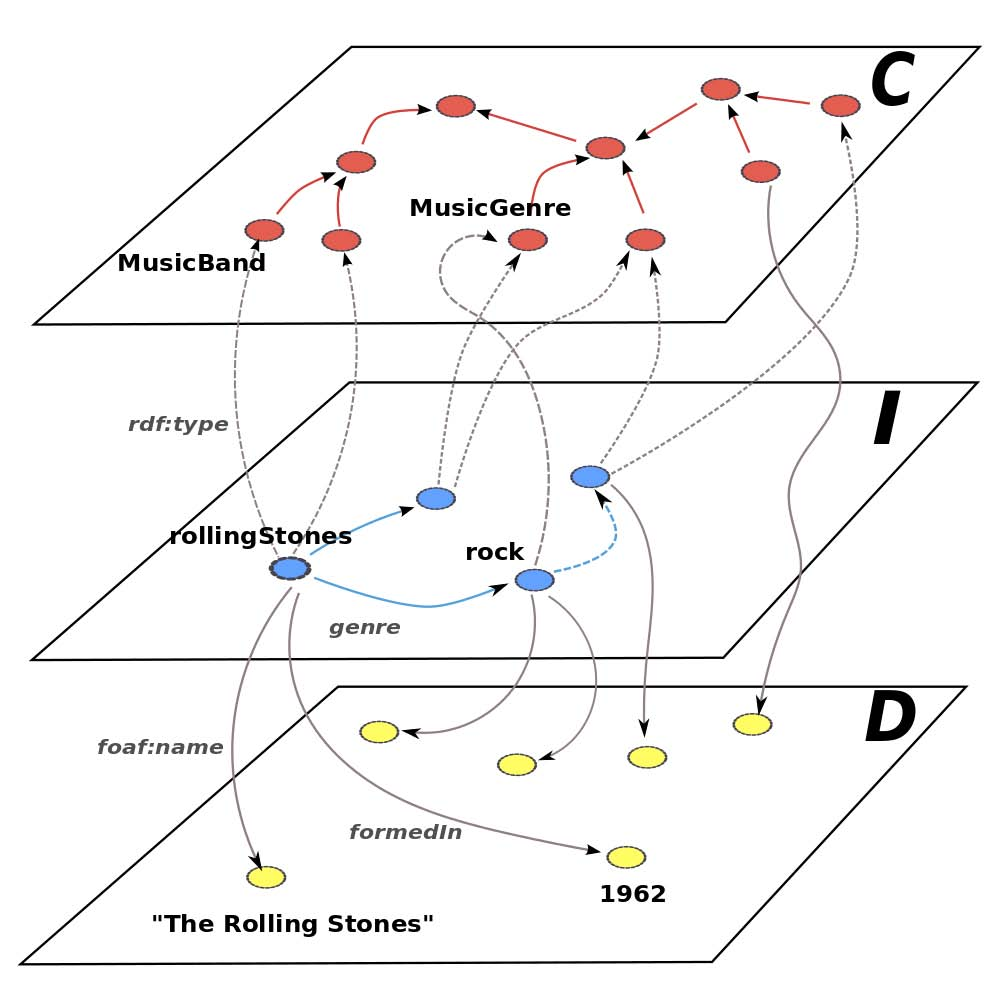
\includegraphics[height=.8\textheight]{instances.png}}
  {\tiny From Harispe et al., Semantic Similarity From Natural
    Language And Ontology Analysis, 2015.}
\end{frame}

\begin{frame}
  \frametitle{Graph-based learning}
  \begin{itemize}
  % \item feature learning on graphs
  %   \pause
  \item e.g., iterated, edge-labeled random walk
    \begin{itemize}
      % \item over instances and classes
    \item walks form {\em sentences}
    \item sentences form a {\em corpus}
    \item feature learning on corpus through Word2Vec (or factorization
      of co-occurrence matrix)
    \item RDF2Vec:
      \url{http://data.dws.informatik.uni-mannheim.de/rdf2vec/}
    \item with support for reasoning over ontologies:
      \url{https://github.com/bio-ontology-research-group/walking-rdf-and-owl}
    \end{itemize}
    \pause
  \item Translational knowledge graph embeddings: TransE, TransR, TransE, HolE, etc.
    \begin{itemize}
    \item analogy- or translation-based
    \item \url{https://github.com/SmartDataAnalytics/PyKEEN}
    \end{itemize}
    \pause
  \item Graph Neural Networks
  \end{itemize}
\end{frame}

\begin{frame}
  \frametitle{Random walks}
  \begin{columns}
    \begin{column}{.6\textwidth}
      \resizebox{1\textwidth}{!}{%
        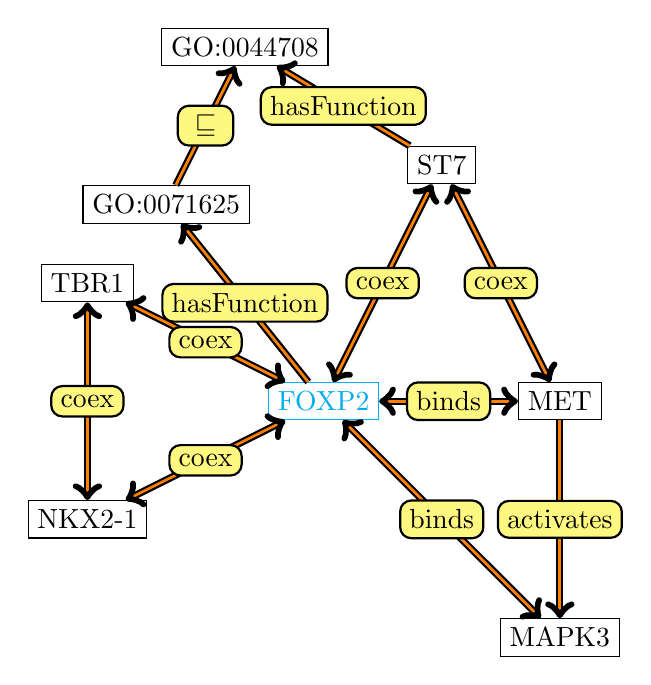
\begin{tikzpicture}
%          \SetUpEdge[lw = 1pt, color = black]
          \GraphInit[vstyle=Shade]
          \tikzset{
            LabelStyle/.style = { rectangle, rounded corners, draw,
              minimum width = 2em, fill = yellow!50,
              text = black },
            VertexStyle/.append style = { inner sep=5pt,
              font = \Large\bfseries},
            EdgeStyle/.append style = {->} }
          
          \SetGraphUnit{5}
          % \tikzset{VertexStyle/.append style={fill}}
          % \tikzset{EdgeStyle/.style={->}}
          \node[draw, color=cyan] (FOXP2) at (0,0) {FOXP2};
          \node[draw] (MET) at (3,0) {MET};
          \node[draw] (ST7) at (1.5,3) {ST7};
          \node[draw] (MAPK3) at (3,-3) {MAPK3};
          \node[draw] (GO0071625) at (-2,2.5) {GO:0071625};
          \node[draw] (GO0044708) at (-1,4.5) {GO:0044708};
          \node[draw] (TBR1) at (-3,1.5) {TBR1};
          \node[draw] (NKX2-1) at (-3,-1.5) {NKX2-1};
          \begin{scope}[/tikz/handle active characters in nodes=false]
          \Edge[label=activates](MET)(MAPK3)
          \Edge[label=hasFunction](FOXP2)(GO0071625)
          \Edge[label=hasFunction](ST7)(GO0044708)
          \Edge[label=$\sqsubseteq$](GO0071625)(GO0044708)

          \tikzset{EdgeStyle/.append style={<->}}
          \Edge[label=binds](FOXP2)(MET)
          \Edge[label=binds](FOXP2)(MAPK3)
          \Edge[label=coex](FOXP2)(TBR1)
          \Edge[label=coex](FOXP2)(NKX2-1)
          \Edge[label=coex](FOXP2)(ST7)
          \Edge[label=coex](MET)(ST7)
          \Edge[label=coex](NKX2-1)(TBR1)
          \end{scope}
          % \tikzset{EdgeStyle/.style={->}}
          % \Edge[label=hf](FOXP2)(GO0044708)
          % \draw[label=binds] (FOXP2) to (MET);
          % \Edge[label=binds](FOXP2)(MET)
          % \Edge[label=activates](MET)(MAPK3)
          % \Edge[label=coexpressed-with](FOXP2)(FOXP4)
          
        \end{tikzpicture}
      }
    \end{column}
    \begin{column}{.4\textwidth}
      \begin{itemize}
      \item FOXP2 is characterized by {\em adjacent} and close nodes
        and edges
      \item different edges may ``transmit'' information differently
      \end{itemize}
    \end{column}
  \end{columns}
      
\end{frame}

\begin{frame}
  \frametitle{Random walks}
%  \frametitle{Neuro-symbolic feature learning}
  \begin{columns}
    \begin{column}{.6\textwidth}
      \resizebox{1\textwidth}{!}{%
        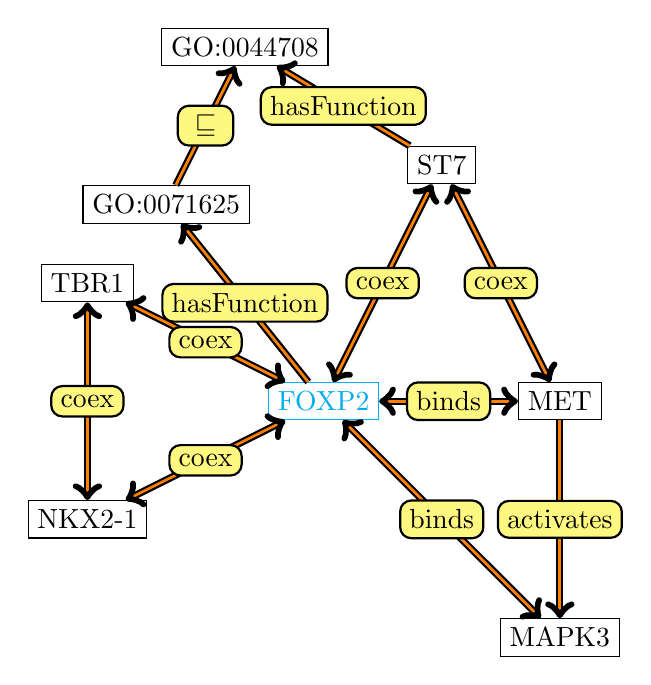
\begin{tikzpicture}
%          \SetUpEdge[lw = 1pt, color = black]
          \GraphInit[vstyle=Shade]
          \tikzset{
            LabelStyle/.style = { rectangle, rounded corners, draw,
              minimum width = 2em, fill = yellow!50,
              text = black },
            VertexStyle/.append style = { inner sep=5pt,
              font = \Large\bfseries},
            EdgeStyle/.append style = {->} }
          
          \SetGraphUnit{5}
          % \tikzset{VertexStyle/.append style={fill}}
          % \tikzset{EdgeStyle/.style={->}}
          \node[draw, color=cyan] (FOXP2) at (0,0) {FOXP2};
          \node[draw] (MET) at (3,0) {MET};
          \node[draw] (ST7) at (1.5,3) {ST7};
          \node[draw] (MAPK3) at (3,-3) {MAPK3};
          \node[draw] (GO0071625) at (-2,2.5) {GO:0071625};
          \node[draw] (GO0044708) at (-1,4.5) {GO:0044708};
          \node[draw] (TBR1) at (-3,1.5) {TBR1};
          \node[draw] (NKX2-1) at (-3,-1.5) {NKX2-1};
          \begin{scope}[/tikz/handle active characters in nodes=false]
          \Edge[label=activates](MET)(MAPK3)
          \Edge[label=hasFunction](FOXP2)(GO0071625)
          \Edge[label=hasFunction](ST7)(GO0044708)
          \Edge[label=$\sqsubseteq$](GO0071625)(GO0044708)

          \tikzset{EdgeStyle/.append style={<->}}
          \Edge[label=binds](FOXP2)(MET)
          \Edge[label=binds](FOXP2)(MAPK3)
          \Edge[label=coex](FOXP2)(TBR1)
          \Edge[label=coex](FOXP2)(NKX2-1)
          \Edge[label=coex](FOXP2)(ST7)
          \Edge[label=coex](MET)(ST7)
          \Edge[label=coex](NKX2-1)(TBR1)
          \end{scope}
          % \tikzset{EdgeStyle/.style={->}}
          % \Edge[label=hf](FOXP2)(GO0044708)
          % \draw[label=binds] (FOXP2) to (MET);
          % \Edge[label=binds](FOXP2)(MET)
          % \Edge[label=activates](MET)(MAPK3)
          % \Edge[label=coexpressed-with](FOXP2)(FOXP4)
          
        \end{tikzpicture}
      }
    \end{column}
    \begin{column}{.4\textwidth}
      \begin{itemize}
      \item precompute the deductive closure:
      \item for all $\phi$: if $\mathcal{KG} \models \phi$, add $\phi$
        to $\mathcal{KG}$
      \end{itemize}
    \end{column}
  \end{columns}
      
\end{frame}

\begin{frame}
  \frametitle{Random walks}
%  \frametitle{Neuro-symbolic feature learning}
  \begin{columns}
    \begin{column}{.6\textwidth}
      \resizebox{1\textwidth}{!}{%
        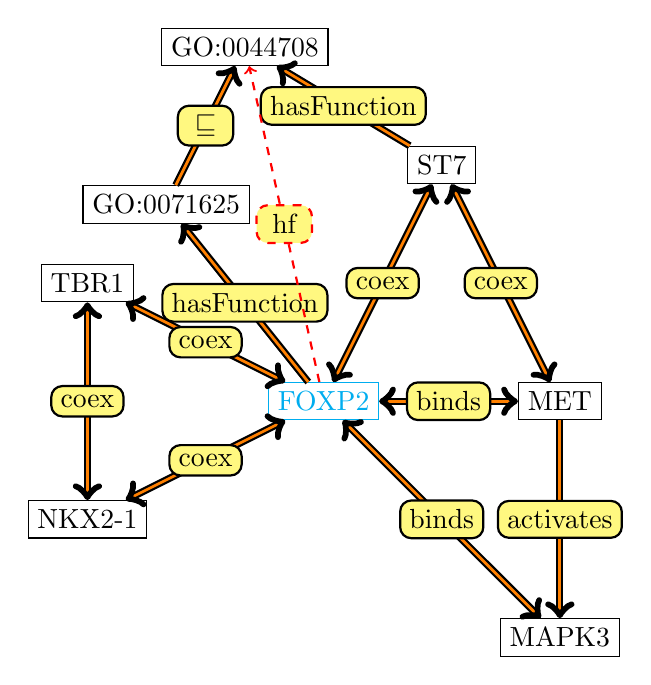
\begin{tikzpicture}
%          \SetUpEdge[lw = 1pt, color = black]
          \GraphInit[vstyle=Shade]
          \tikzset{
            LabelStyle/.style = { rectangle, rounded corners, draw,
              minimum width = 2em, fill = yellow!50,
              text = black },
            VertexStyle/.append style = { inner sep=5pt,
              font = \Large\bfseries},
            EdgeStyle/.append style = {->} }
          
          \SetGraphUnit{5}
          % \tikzset{VertexStyle/.append style={fill}}
          % \tikzset{EdgeStyle/.style={->}}
          \node[draw, color=cyan] (FOXP2) at (0,0) {FOXP2};
          \node[draw] (MET) at (3,0) {MET};
          \node[draw] (ST7) at (1.5,3) {ST7};
          \node[draw] (MAPK3) at (3,-3) {MAPK3};
          \node[draw] (GO0071625) at (-2,2.5) {GO:0071625};
          \node[draw] (GO0044708) at (-1,4.5) {GO:0044708};
          \node[draw] (TBR1) at (-3,1.5) {TBR1};
          \node[draw] (NKX2-1) at (-3,-1.5) {NKX2-1};
          \begin{scope}[/tikz/handle active characters in nodes=false]
          \Edge[label=activates](MET)(MAPK3)
          \Edge[label=hasFunction](FOXP2)(GO0071625)
          \Edge[label=hasFunction](ST7)(GO0044708)
          \Edge[label=$\sqsubseteq$](GO0071625)(GO0044708)

          \tikzset{EdgeStyle/.append style={<->}}
          \Edge[label=binds](FOXP2)(MET)
          \Edge[label=binds](FOXP2)(MAPK3)
          \Edge[label=coex](FOXP2)(TBR1)
          \Edge[label=coex](FOXP2)(NKX2-1)
          \Edge[label=coex](FOXP2)(ST7)
          \Edge[label=coex](MET)(ST7)
          \Edge[label=coex](NKX2-1)(TBR1)

          \tikzset{EdgeStyle/.style={->}}
          \Edge[label=hf, color=red, style=dashed](FOXP2)(GO0044708)
          \end{scope}
          % \tikzset{EdgeStyle/.style={->}}
          % \Edge[label=hf](FOXP2)(GO0044708)
          % \draw[label=binds] (FOXP2) to (MET);
          % \Edge[label=binds](FOXP2)(MET)
          % \Edge[label=activates](MET)(MAPK3)
          % \Edge[label=coexpressed-with](FOXP2)(FOXP4)
          
        \end{tikzpicture}
      }
    \end{column}
    \begin{column}{.4\textwidth}
      \begin{itemize}
      \item precompute the deductive closure:
      \item for all $\phi$: if $\mathcal{KG} \models \phi$, add $\phi$
        to $\mathcal{KG}$
      \end{itemize}
    \end{column}
  \end{columns}
      
\end{frame}


\begin{frame}
  \frametitle{Random walks}
%  \frametitle{Neuro-symbolic feature learning}
  \begin{columns}
    \begin{column}{.6\textwidth}
      \resizebox{1\textwidth}{!}{%
        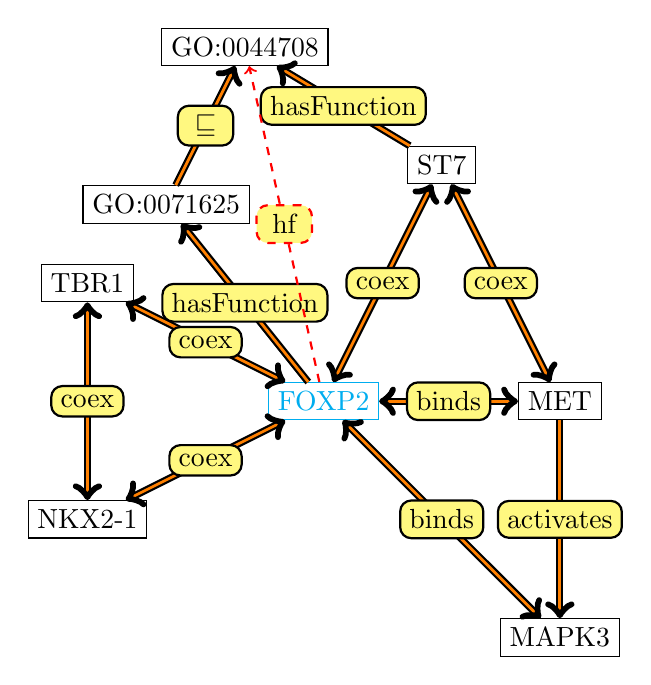
\begin{tikzpicture}
%          \SetUpEdge[lw = 1pt, color = black]
          \GraphInit[vstyle=Shade]
          \tikzset{
            LabelStyle/.style = { rectangle, rounded corners, draw,
              minimum width = 2em, fill = yellow!50,
              text = black },
            VertexStyle/.append style = { inner sep=5pt,
              font = \Large\bfseries},
            EdgeStyle/.append style = {->} }
          
          \SetGraphUnit{5}
          % \tikzset{VertexStyle/.append style={fill}}
          % \tikzset{EdgeStyle/.style={->}}
          \node[draw, color=cyan] (FOXP2) at (0,0) {FOXP2};
          \node[draw] (MET) at (3,0) {MET};
          \node[draw] (ST7) at (1.5,3) {ST7};
          \node[draw] (MAPK3) at (3,-3) {MAPK3};
          \node[draw] (GO0071625) at (-2,2.5) {GO:0071625};
          \node[draw] (GO0044708) at (-1,4.5) {GO:0044708};
          \node[draw] (TBR1) at (-3,1.5) {TBR1};
          \node[draw] (NKX2-1) at (-3,-1.5) {NKX2-1};
          \begin{scope}[/tikz/handle active characters in nodes=false]
          \Edge[label=activates](MET)(MAPK3)
          \Edge[label=hasFunction](FOXP2)(GO0071625)
          \Edge[label=hasFunction](ST7)(GO0044708)
          \Edge[label=$\sqsubseteq$](GO0071625)(GO0044708)

          \tikzset{EdgeStyle/.append style={<->}}
          \Edge[label=binds](FOXP2)(MET)
          \Edge[label=binds](FOXP2)(MAPK3)
          \Edge[label=coex](FOXP2)(TBR1)
          \Edge[label=coex](FOXP2)(NKX2-1)
          \Edge[label=coex](FOXP2)(ST7)
          \Edge[label=coex](MET)(ST7)
          \Edge[label=coex](NKX2-1)(TBR1)

          \tikzset{EdgeStyle/.style={->}}
          \Edge[label=hf, color=red, style=dashed](FOXP2)(GO0044708)
          \end{scope}
          % \draw[label=binds] (FOXP2) to (MET);
          % \Edge[label=binds](FOXP2)(MET)
          % \Edge[label=activates](MET)(MAPK3)
          % \Edge[label=coexpressed-with](FOXP2)(FOXP4)
          
        \end{tikzpicture}
      }
    \end{column}
    \begin{column}{.4\textwidth}
      \begin{itemize}
      \item Exploring the graph:
        \pause
      \item :FOXP2 :binds :MET :coex :ST7 :hasFunction GO:0044708
        \pause
      \item :FOXP2 :hasFunction GO:0071625 subClassOf GO:0044708
        \pause
      \item :FOXP2 :coex :TBR1 :coex :NKX2-1 :coex :TBR1 :coex ...
      \end{itemize}
    \end{column}
  \end{columns}
\end{frame}

\begin{frame}
  \frametitle{Word2Vec and Random Walks}
  \begin{itemize}
  \item random walks ``flatten'' a graph
    \begin{itemize}
    \item walks capture node neighborhood
    \item and generate a ``corpus''
    \end{itemize}
  \item random walks capture graph ``structure''
    \begin{itemize}
    \item in ABox and TBox
    \item hub-nodes, communities, etc.
    \item determine ``importance'' of nodes
    \end{itemize}
  \item embeddings capture co-occurrence
    \begin{itemize}
    \item similar graph neighborhood $\Rightarrow$ similar
      co-occurrence $\Rightarrow$ similar vector
    \end{itemize}
  \item embeddings generate ``feature'' vectors
    \begin{itemize}
    \item functions from symbols (words, labels) into $\Re^n$
    \end{itemize}
  \end{itemize}
\end{frame}

\begin{frame}
  \frametitle{Translating embeddings}
  \centerline{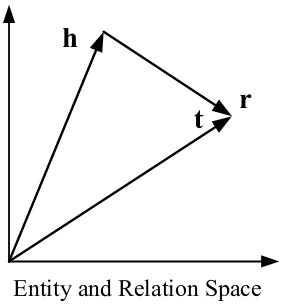
\includegraphics[width=.7\textwidth]{transe-figure.png}}
\end{frame}

\begin{frame}
  \frametitle{Translating embeddings}
  \begin{columns}
    \begin{column}{.6\textwidth}
      \resizebox{1\textwidth}{!}{%
        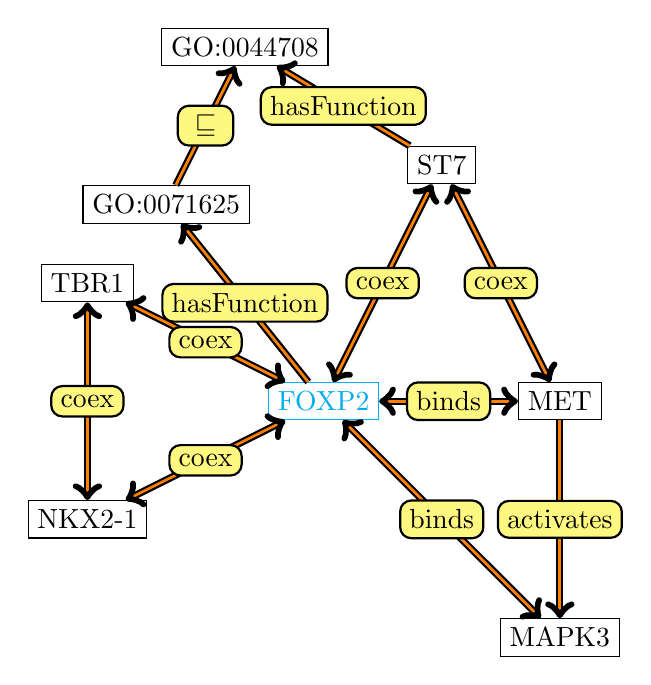
\begin{tikzpicture}
%          \SetUpEdge[lw = 1pt, color = black]
          \GraphInit[vstyle=Shade]
          \tikzset{
            LabelStyle/.style = { rectangle, rounded corners, draw,
              minimum width = 2em, fill = yellow!50,
              text = black },
            VertexStyle/.append style = { inner sep=5pt,
              font = \Large\bfseries},
            EdgeStyle/.append style = {->} }
          
          \SetGraphUnit{5}
          % \tikzset{VertexStyle/.append style={fill}}
          % \tikzset{EdgeStyle/.style={->}}
          \node[draw, color=cyan] (FOXP2) at (0,0) {FOXP2};
          \node[draw] (MET) at (3,0) {MET};
          \node[draw] (ST7) at (1.5,3) {ST7};
          \node[draw] (MAPK3) at (3,-3) {MAPK3};
          \node[draw] (GO0071625) at (-2,2.5) {GO:0071625};
          \node[draw] (GO0044708) at (-1,4.5) {GO:0044708};
          \node[draw] (TBR1) at (-3,1.5) {TBR1};
          \node[draw] (NKX2-1) at (-3,-1.5) {NKX2-1};
          \begin{scope}[/tikz/handle active characters in nodes=false]
          \Edge[label=activates](MET)(MAPK3)
          \Edge[label=hasFunction](FOXP2)(GO0071625)
          \Edge[label=hasFunction](ST7)(GO0044708)
          \Edge[label=$\sqsubseteq$](GO0071625)(GO0044708)

          \tikzset{EdgeStyle/.append style={<->}}
          \Edge[label=binds](FOXP2)(MET)
          \Edge[label=binds](FOXP2)(MAPK3)
          \Edge[label=coex](FOXP2)(TBR1)
          \Edge[label=coex](FOXP2)(NKX2-1)
          \Edge[label=coex](FOXP2)(ST7)
          \Edge[label=coex](MET)(ST7)
          \Edge[label=coex](NKX2-1)(TBR1)
          \end{scope}
          % \tikzset{EdgeStyle/.style={->}}
          % \Edge[label=hf](FOXP2)(GO0044708)
          % \draw[label=binds] (FOXP2) to (MET);
          % \Edge[label=binds](FOXP2)(MET)
          % \Edge[label=activates](MET)(MAPK3)
          % \Edge[label=coexpressed-with](FOXP2)(FOXP4)
          
        \end{tikzpicture}
      }
    \end{column}
    \begin{column}{.4\textwidth}
      \begin{itemize}
        \pause
      \item FOXP2 + binds = MET
        \pause
      \item MET + activates = MAPK3
        \pause
      \item MET + binds = FOXP2
        \pause
      \item ST7 + hasFunction = {\tt GO:0044708}
        \pause
      \item ...
      \end{itemize}
    \end{column}
  \end{columns}
\end{frame}

\begin{frame}
  \frametitle{Translating embeddings}
  \begin{columns}
    \begin{column}{.6\textwidth}
      \resizebox{1\textwidth}{!}{%
        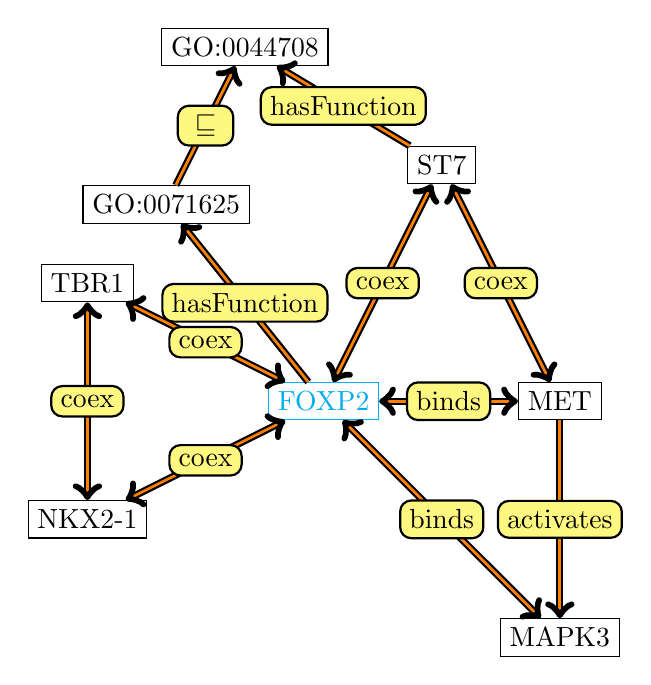
\begin{tikzpicture}
%          \SetUpEdge[lw = 1pt, color = black]
          \GraphInit[vstyle=Shade]
          \tikzset{
            LabelStyle/.style = { rectangle, rounded corners, draw,
              minimum width = 2em, fill = yellow!50,
              text = black },
            VertexStyle/.append style = { inner sep=5pt,
              font = \Large\bfseries},
            EdgeStyle/.append style = {->} }
          
          \SetGraphUnit{5}
          % \tikzset{VertexStyle/.append style={fill}}
          % \tikzset{EdgeStyle/.style={->}}
          \node[draw, color=cyan] (FOXP2) at (0,0) {FOXP2};
          \node[draw] (MET) at (3,0) {MET};
          \node[draw] (ST7) at (1.5,3) {ST7};
          \node[draw] (MAPK3) at (3,-3) {MAPK3};
          \node[draw] (GO0071625) at (-2,2.5) {GO:0071625};
          \node[draw] (GO0044708) at (-1,4.5) {GO:0044708};
          \node[draw] (TBR1) at (-3,1.5) {TBR1};
          \node[draw] (NKX2-1) at (-3,-1.5) {NKX2-1};
          \begin{scope}[/tikz/handle active characters in nodes=false]
          \Edge[label=activates](MET)(MAPK3)
          \Edge[label=hasFunction](FOXP2)(GO0071625)
          \Edge[label=hasFunction](ST7)(GO0044708)
          \Edge[label=$\sqsubseteq$](GO0071625)(GO0044708)

          \tikzset{EdgeStyle/.append style={<->}}
          \Edge[label=binds](FOXP2)(MET)
          \Edge[label=binds](FOXP2)(MAPK3)
          \Edge[label=coex](FOXP2)(TBR1)
          \Edge[label=coex](FOXP2)(NKX2-1)
          \Edge[label=coex](FOXP2)(ST7)
          \Edge[label=coex](MET)(ST7)
          \Edge[label=coex](NKX2-1)(TBR1)
          \end{scope}
          % \tikzset{EdgeStyle/.style={->}}
          % \Edge[label=hf](FOXP2)(GO0044708)
          % \draw[label=binds] (FOXP2) to (MET);
          % \Edge[label=binds](FOXP2)(MET)
          % \Edge[label=activates](MET)(MAPK3)
          % \Edge[label=coexpressed-with](FOXP2)(FOXP4)
          
        \end{tikzpicture}
      }
    \end{column}
    \begin{column}{.4\textwidth}
      \begin{itemize}
      \item FOXP2 + binds - MET = 0
      \item MAP + activates - MAPK3 = 0
      \item MET + binds - FOXP2 = 0
      \item ST7 + hasFunction - {\tt GO:0044708} = 0
      \item ...
      \end{itemize}
    \end{column}
  \end{columns}
\end{frame}

\begin{frame}
  \frametitle{Ontologies: axioms, not graphs!}
    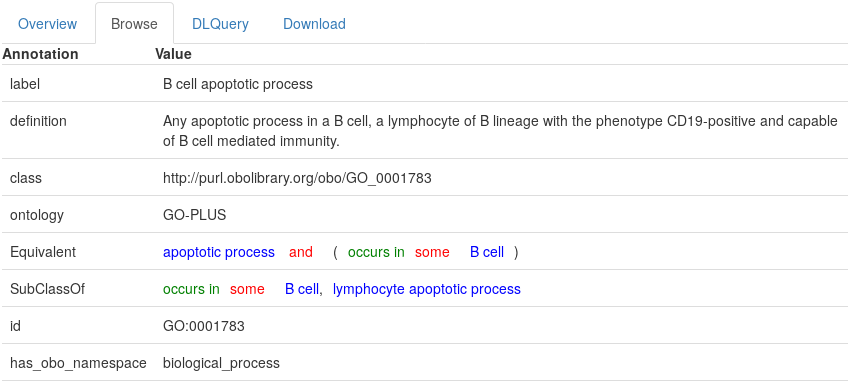
\includegraphics[width=1\textwidth]{bcellapoptosis.png}
\end{frame}

\begin{frame}
  \frametitle{Ontologies: axioms, not graphs!}
  Gene Ontology:
  \begin{itemize}
  \item {\tt behavior DisjointWith: 'developmental process'}
  \item {\tt behavior SubclassOf: only-in-taxon some metazoa}
  \item {\tt 'cell proliferation' DisjointWith: in-taxon some fungi}
  \item {\tt 'cell growth' EquivalentTo: growth and ('results in
      growth of' some cell)}
  \item ...
  \end{itemize}
\end{frame}

\begin{frame}
  \frametitle{Onto2Vec}
  \centerline{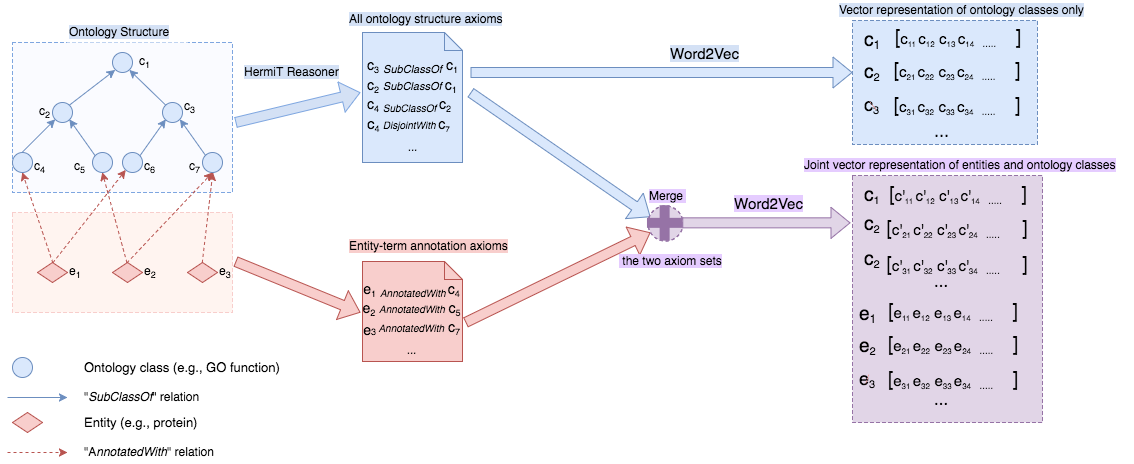
\includegraphics[width=\textwidth]{onto2vecflow.png}}
\end{frame}

\begin{frame}
  \frametitle{Word2Vec}
  Maximize:
  \begin{equation}
    \frac{1}{N} \sum_{n=1}^{N} \sum_{-c\leq j \leq c, j\not=
      0} \log p(w_{n+j}|w_n)
  \end{equation}
  with
  \begin{equation}
    p(w_o | w_i) = \frac{\exp({v'_{w_o}}^T v_{w_i})}{\sum_{w=1}^{W}
      \exp({v'_{w}}^T v_{w_i})}
  \end{equation}
  (at least conceptually; different strategies are used to approximate Eqn. 2)
\end{frame}

\begin{frame}
  \frametitle{Word2Vec}
  \centerline{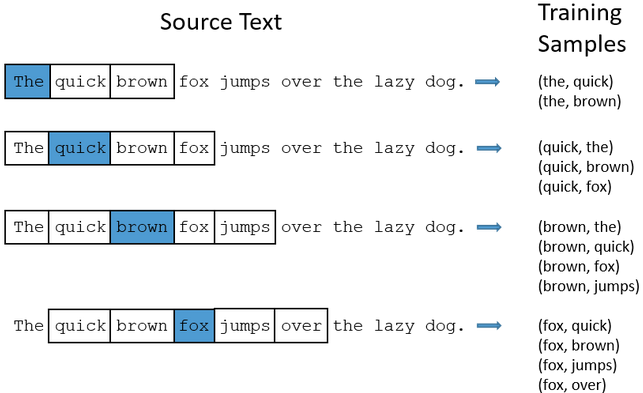
\includegraphics[width=\textwidth]{word2vec-example.png}}
\end{frame}

\begin{frame}
  \frametitle{Combination with text}
  \begin{itemize}
  \item ontologies contain more than axioms:
    \begin{itemize}
    \item labels, synonyms, definitions, authors, etc.
    \end{itemize}
  \item Description Logic axioms != natural language
  \item transfer learning: learn on one domain/task, apply to another
    \begin{itemize}
    \item e.g.: learn on literature, apply to ontologies
    \item words have ``meaning'' in literature, Description Logic
      symbols have ``meaning'' in ontology axioms
    \end{itemize}
  \item Ontologies Plus Annotations 2 Vec (OPA2Vec) combines both
  \end{itemize}
\end{frame}

\begin{frame}
  \frametitle{Ontologies Plus Annotations 2 Vec}
  \centerline{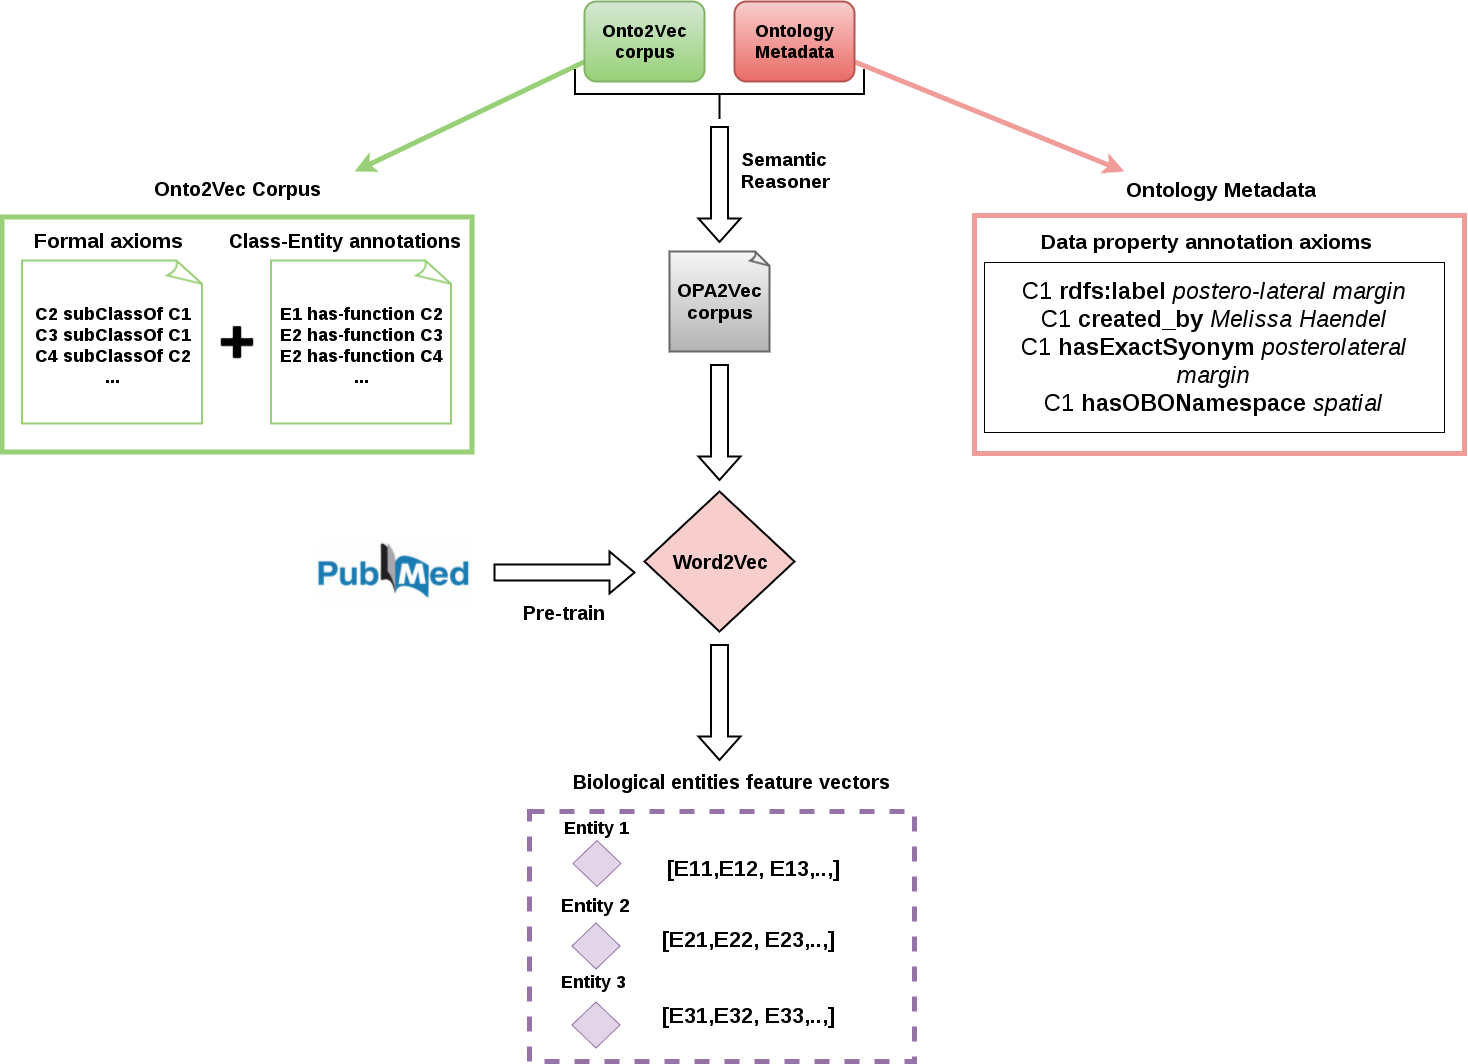
\includegraphics[width=1\textwidth]{opaworkflow16.png}}
\end{frame}

\begin{frame}
  \frametitle{OPA2Vec}
  \begin{itemize}
  \item \url{https://github.com/bio-ontology-research-group/opa2vec}
  \item command line tool
    \begin{itemize}
    \item input: OWL ontology, set of entities with annotations/associations
    \item output: vectors for each class and entity
    \end{itemize}
  \item includes Elk and HermiT
  \item limitations: word-based
    \begin{itemize}
    \item completely ignores any semantics!
    \end{itemize}
  \end{itemize}
\end{frame}

\begin{frame}
  \frametitle{How to build ``semantic'' embeddings}
  \begin{itemize}
  \item none of the models discussed above are truly ``semantic''
    \begin{itemize}
    \item all syntactic
    \item graph-based or based on axioms
    \end{itemize}
    \pause
  \item what do we actually mean by ``semantics''?
    \begin{itemize}
    \pause
    \item formal definition of ``truth'' relies on ``models''
    \pause
    \item universal algebra over formal languages (with signature
      $\Sigma$)
    \end{itemize}
  \end{itemize}
\end{frame}

\begin{frame}
  \frametitle{Description Logic EL++}
  \centering
  \resizebox{.8\textwidth}{!}{
    
    \begin{tabular}{|p{1.7cm}|c|p{3.7cm}|}
      \hline
      {\bf} Name & Syntax & Semantics \\
      \hline
      top & $\top$ & $\Delta^{\mathcal{I}}$ \\
    \hline
    bottom & $\bot$ & $\emptyset$ \\
    \hline
    nominal & $\{ a \} $ & $\{ a^{\mathcal{I}} \}$ \\
    \hline
    conjunction & $C \sqcap D$ & $ C^{\mathcal{I}} \cap
                                 D^{\mathcal{I}}$ \\
    \hline
    existential restriction & $\exists r.C$ & $ \{ x \in
                                              \Delta^{\mathcal{I}} |
                                              \exists y \in
                                              \Delta^{\mathcal{I}} :
                                              (x,y) \in
                                              r^{\mathcal{I}} \land y
                                              \in C^{\mathcal{I}} \} $
    \\
    \hline
    generalized concept inclusion & $C \sqsubseteq D$ &
                                                        $C^{\mathcal{I}}
                                                        \subseteq
                                                        D^{\mathcal{I}}$
    \\
    \hline
    role inclusion & $r_1 \circ ... \circ r_n \sqsubseteq r$ &
                                                               $r_1^{\mathcal{I}}
                                                               \circ
                                                               ... \circ
                                                               r_n^{\mathcal{I}}
                                                               \subseteq
                                                               r^{\mathcal{I}}$
    \\
    \hline
    
  \end{tabular}
}
\end{frame}

\begin{frame}
  \frametitle{Models}
  \begin{itemize}
  \item Interpretations and $\Sigma$-structures
  \item Model $\mathfrak{A}$ of a formula $\phi$: $\phi$ is true in
    $\mathfrak{A}$ ($\mathfrak{A} \models \phi$) 
  \item Theory $T$: set of formulas
  \item $\mathfrak{A}$ is a model of $T$ if $\mathfrak{A}$ is a model
    of all formulas in $T$
  \item Ontologies are (special kinds of) theories
  \end{itemize}
\end{frame}

\begin{frame}
  \frametitle{EL Embeddings}
  \begin{itemize}
  \item given a theory/ontology $T$ with signature $\Sigma(T)$
  \item aim: find $f_e: \Sigma(T) \mapsto \Re^n$ s.t. $f_e(\Sigma(T))$
    is a model of $T$ ($f_e(\Sigma(T)) \models T$)
    \pause
  \item more general: find an algorithm that maps symbols (signatures)
    into $\Re^n$ so that the {\em semantics} of the symbol (expressed
    through axioms and explicit in model structures) is preserved
    \begin{itemize}
    \item or: the embedding function {\em is} an interpretation function
    \end{itemize}

    \pause
  \item any consistent \el  theory has infinite models
    \pause
  \item any consistent \el  theory has models in $\mathbb{R}^n$
    (Loewenheim-Skolem, upwards; compactness)
  \end{itemize}
\end{frame}

\begin{frame}
  \frametitle{Key idea}
  \begin{itemize}
  \item for all $r \in \Sigma(T)$ and $C \in \Sigma(T)$, define
    $f_e(r)$ and $f_e(C)$
  \item $f_e(C)$ maps to points in an open $n$-ball such that
    $f_e(C) = C^{\mathcal{I}}$:
    $C^{\mathcal{I}} = \{ x \in \mathbb{R}^n | \norm{f_e(C) - x} <
    r_e(C) \}$
    \begin{itemize}
    \item these are the {\em extension} of a class in $\Re^n$
    \end{itemize}
  \item $f_e(r)$ maps a binary relation $r$ to a vector such that
    % the set of tuples ($\mathbb{R}^n \times \mathbb{R}^n$) with
    % $f_e(r) = r^{\mathcal{I}}$:
    $r^{\mathcal{I}} = \{ (x,y) | x + f_e(r) = y \}$
    \begin{itemize}
    \item that's the TransE property for {\em individuals}
    \end{itemize}
  \item use the axioms in $T$ as constraints
  \end{itemize}
\end{frame}

\begin{frame}
  \frametitle{Algorithm}
  \begin{itemize}
  \item normalize the theory:
    \begin{itemize}
    \item every \el theory can be expressed using four normal forms
      (Baader et al., 2005)
    \end{itemize}
  \item eliminate the ABox: replace each individual symbol with a
    singleton class: $a$ becomes $\{a\}$
  \item rewrite relation assertions $r(a,b)$ and class
    assertions $C(a)$ as $\{ a \} \sqsubseteq \exists r.\{ b \}$ and
    $\{ a \} \sqsubseteq C$
    \begin{itemize}
    \item something to remember for the next class-vs-instance discussion?
    \end{itemize}
  \item normalization rules to generate:
    \begin{itemize}
    \item $C \sqsubseteq D$
    \item $C \sqcap D \sqsubseteq E$
    \item $C \sqsubseteq \exists R.D$
    \item $\exists R.C \sqsubseteq D$
    \end{itemize}
  \end{itemize}
\end{frame}

\begin{frame}
  \frametitle{Algorithm: loss functions}
  \begin{equation}
    \label{eqn:nf1}
    \begin{split}
      & loss_{C \sqsubseteq D}(c,d) = \\
      & \max(0, \norm{f_\eta(c) - f_\eta(d)} + r_\eta(c) - r_\eta(d) - \gamma) \\
      & + |\norm{f_\eta(c)} - 1| + |\norm{f_\eta(d)} - 1|
    \end{split}
  \end{equation}
\end{frame}

\begin{frame}
  \frametitle{Algorithm: loss functions}
  Let
  $h=\frac{r_\eta(c)^2-r_\eta(d)^2+\norm{f_\eta(c) -
      f_\eta(d)}^2}{2\norm{f_\eta(c) - f_\eta(d)}}$, then the center and
  radius of the smallest $n$-ball containing the intersection of
  $\eta(C)$ and $\eta(D)$ are
  $f_\eta(c)+\frac{h}{\norm{f_\eta(c) -
      f_\eta(d)}}(f_\eta(d)-f_\eta(c))$ and $\sqrt{r_\eta(c)^2-h^2}$.
\end{frame}

\begin{frame}
  \frametitle{Algorithm: loss functions}
  \begin{equation}
    \label{eqn:nf3}
    \begin{split}
      & loss_{C \sqsubseteq \exists R.D}(c,d,r) = \\
      & \max(0, \norm{f_\eta(c) + f_\eta(r) - f_\eta(d)}  + r_\eta(c) - r_\eta(d) - \gamma) \\
      & + |\norm{f_\eta(c)} - 1| + |\norm{f_\eta(d)} - 1|
    \end{split}
  \end{equation}
\end{frame}

\begin{frame}
  \frametitle{Algorithm: loss functions}
  \begin{equation}
    \label{eqn:nf4}
    \begin{split}
      & loss_{\exists R.C \sqsubseteq D}(c,d,r) = \\
      & \max(0, \norm{f_\eta(c) - f_\eta(r) - f_\eta(d)} - r_\eta(c) - r_\eta(d) - \gamma) \\
      & + |\norm{f_\eta(c)} - 1| + |\norm{f_\eta(d)} - 1|
    \end{split}
  \end{equation}
\end{frame}

\begin{frame}
  \frametitle{Algorithm: loss functions}
  \begin{equation}
    \label{eqn:disjoint}
    \begin{split} 
      &loss_{C \sqcap D \sqsubseteq \bot}(c,d,e) = \\
      & \max(0, r_\eta(c) + r_\eta(d) - \norm{f_\eta(c) - f_\eta(d)} + \gamma) \\
      & + |\norm{f_\eta(c)} - 1| + |\norm{f_\eta(d)} - 1|
    \end{split}
  \end{equation}
\end{frame}

\begin{frame}
  \frametitle{Algorithm: loss functions}
  \centerline{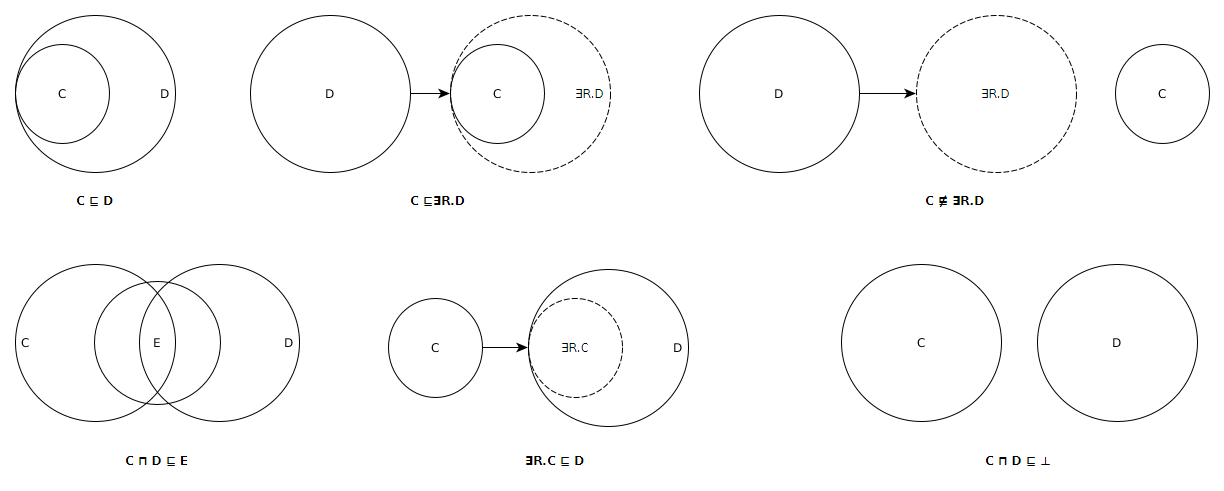
\includegraphics[width=1\textwidth]{ellosses.png}}
\end{frame}

\begin{frame}
  \frametitle{EL Embeddings}
  \begin{eqnarray}
    & Male & \sqsubseteq Person \\
    & Female & \sqsubseteq Person \\
    & Father & \sqsubseteq Male \\
    & Mother & \sqsubseteq Female \\
    & Father & \sqsubseteq Parent \\
    & Mother & \sqsubseteq Parent \\
    & Female \sqcap Male & \sqsubseteq \bot \\
    & Female \sqcap Parent & \sqsubseteq Mother \\
    & Male \sqcap Parent & \sqsubseteq Father \\
    & \exists hasChild.Person & \sqsubseteq Parent \\
    & Parent & \sqsubseteq Person \\
    & Parent & \sqsubseteq \exists hasChild.\top
               \label{famlast}
               % & Person & \sqsubseteq \top
  \end{eqnarray}
\end{frame}

\begin{frame}
  \frametitle{EL Embeddings}
  \centerline{\animategraphics[loop,controls,width=.7\textwidth]{12}{embeds-frame-}{0}{99}}
  \begin{itemize}
  \item model with $\Delta = R^n$
  \item support quantifiers, negation, conjunction,...
  \end{itemize}
  {\tiny IJCAI 2019}
\end{frame}


\end{document}
%%% Local Variables:
%%% mode: latex
%%% TeX-master: t
%%% End:
